%!TEX root = main.tex


\documentclass[titlepage, twoside]{article}

\usepackage{lipsum}
\usepackage[pdftex]{graphicx}
\usepackage[margin=1.5in]{geometry}
\usepackage[english]{babel}
   \addto{\captionsenglish}{\renewcommand{\bibname}{Works Cited}}
\usepackage{listings}
\usepackage{amsthm}
\usepackage{amssymb}
\usepackage{framed} 
\usepackage{amsmath}
\usepackage{titling}
\usepackage{amssymb}
\usepackage{relsize}
\usepackage{tikz}
\usepackage{xr}

\usetikzlibrary{decorations.pathreplacing}
\usepackage[colorinlistoftodos]{todonotes}

% margins
\usepackage{bm}

% references
\usepackage{varioref}
\renewcommand\refname{Works Cited}



%%%%%%%%%%%%%%%
% MATH
%%%%%%%%%%%%%%%

\numberwithin{equation}{subsection}
\newcommand{\BlackBox}{\rule{1.5ex}{1.5ex}}  % end of proof
\newtheorem{example}{Example} 
\newtheorem{theorem}{Theorem}
\newtheorem{lemma}[theorem]{Lemma} 
\newtheorem{proposition}[theorem]{Proposition} 
\newtheorem{remark}[theorem]{Remark}
\newtheorem{corollary}[theorem]{Corollary}
\newtheorem{definition}[theorem]{Definition}
\newtheorem{conjecture}[theorem]{Conjecture}
\newtheorem{axiom}[theorem]{Axiom}
\newcommand{\Sum}{\mathlarger{\mathlarger{\sum}}}

\numberwithin{theorem}{subsection}

\newcommand{\rotB}{\scalebox{-1}[1]{B}}
%%%%%%%%%%%%%%%


\newcommand{\subtitle}[1]{%
  \posttitle{%
    \par\end{center}
    \begin{center}\large#1\end{center}
    \vskip0.5em}%
}

\usepackage{float}

\newcommand{\nosection}[1]{%
  \refstepcounter{section}%
  \addcontentsline{toc}{section}{\protect\numberline{\thesection}#1}%
  \markright{#1}}
\newcommand{\unit}[1]{\ensuremath{\, \mathrm{#1}}}

\usepackage{fancyhdr}

\pagestyle{fancy}
\fancyhead[L]{Functional Neural Networks}
\fancyhead[CO]{Weierstrass Approximation}
\fancyhead[CE]{William Guss}
\fancyhead[R]{\thepage}
\fancyfoot[LR]{}
\fancyfoot[C]{}
\usepackage{csquotes}
\numberwithin{equation}{subsection}


%%%%%%%%%%%%%%%%%%
%BIBLIOGRAPHY
%%%%%%%%%%%%%%%%%%
\usepackage{csquotes}
\usepackage[style=ieee, backend=biber]{biblatex}
\addbibresource{FNN.bib}
\DefineBibliographyStrings{english}{
  references = {Bibliography},
}
\def\layersep{2cm}



\begin{document}
\title{Generalized Artifical Neural Networks}
\subtitle{Approximated by Weierstrass Polynomials}
\author{
  Guss, William\\
  \texttt{wguss@berkeley.edu}
}
\date{\today}
\maketitle
\pagenumbering{roman}
\thispagestyle{empty}

\begin{abstract}
%!TEX root = main.tex
In this paper we consider the traditional model of feed-forward neural networks proposed in (McCulloch and Pitts, 1949), and using intuitions developed in (Neal, 1994) we propose a method generalizing discrete neural networks as follows. In the standardized case, neural mappings $\mathcal{N}: \mathbb{R}^n \to [0,1]^m$ have little meaning when $n \to \infty$. Thus we consider a new construction $\mathcal{F}: \mathcal{X} \to \mathcal{Y}$ where the domain and codomain of $\mathcal{N}$ become infinite dimensional Hilbert spaces, namely the set of quadratically Lebesgue integrable functions $L^2$ over a real interval $E$ and $[0,1]$ respectively. The derivation of this construction is intuitively similar to that of Lebesgue integration; that is, $\sum_i \sigma_i w_{ij} \to \int_{E\subset\mathbb{R}}\sigma(i)w(i,j)\ d\mu(s)$. 

After establishing a proper family of "functional neural networks" $\mathcal{F}$, we show that $\mathcal{N}$ are a specific class of functional neural networks under specific constraints. More specifically in our first lemma, we prove that $\mathcal{F} \equiv \mathcal{N}$ for piecewise constant weight functions $w(i,j)$. Having done so, we then attempt to find an analogue to Cybenko's theorem of universal approximation for neural networks. Firstly, we prove as a corollary of the Weierstrass approximation theorem, that $w(i,j)$ can approximate a function,$f:E\to[0,1]$, satisfying $\left\|\mathcal{F}\xi - f(\xi)\right\|_\infty \to 0$. As a byproduct of the proof, we also establish a closed-form definition for the satisfying $w(i,j)$ and thereby through our first lemma provide novel insight into the actual form of the weight matrix $[w_{ij}]$ for trained $\mathcal{N}$. Finally we propose a universal approximation theorem for functional neural networks; that is, we show through the Riesz Representation Theorem that $\mathcal{F}$ approximates any bounded linear operator on $\mathcal{X}$.

In conclusion, we create a practical analogue of the error-backpropagation algorithm, and implement functional neural networks using Simpson’s rule. We suggest that functional neural networks represent an interesting opportunity for the implementation of machine learning systems modeling functional transformation.
\end{abstract}

\newpage
  \thispagestyle{empty}
  \tableofcontents

\pagenumbering{arabic}

%!TEX root = main.tex
\section{Introduction }
Machine learning is an emerging field that deals with the development of algorithms which can predict and classify novelties based on a set of prior “intuitions” \cite{mlsurvey}. The field incorporates ideas from biology, computer science, numerical analysis, and statistics. In recent years machine learning has entered the main stream through web services like Google, Facebook, and Amazon. There is an incentive from both academia and industry to expand machine learning techniques and applications. 

One of the most popular algorithms of the field is the artificial neural network (ANN). Although there are numerous mathematical interpretations of neural networks, we will primarily focus on the expansion of one type, feed-forward neural networks. As ANNs are based off the structure of biological neurons, a biological approach is necessary to understand this interpretation.
\subsection{Biological Neuron}
A single neuron consists of the cell body (the soma), the dendrites, and the axon. Mathematically we wish to examine the process of neural activation, the events which lead to the excitation of the axon. Consider a neuron that has activated anterior neurons (those which are connected dendritically); that is, the neuron is receiving input along all of its dendrites. These electrical inputs propagate through the dendrites and become integrated on the soma as electrical membrane potential \cite{griffith}. The soma then acts as the primary computational unit and activates the axon when a threshold of input activity is reached. More specifically, when a membrane potential of about -60 mV is reached on the soma, the hillock zone, or axon hillock, activates the axon by applying proteins to an ion channel which creates action potential along the axon \cite{bioneuron}.
\subsection{Artificial Neurons}
\begin{figure}
\centering
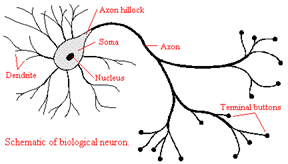
\includegraphics{neuron}
\caption{A biological neuron \cite{neuralimage}.}
\end{figure}
    With this in mind it is now possible to construct a mathematical model of an artificial neuron. Let \( A_j, P_j\) be the set of anterior and posterior neurons of a neuron, \(j\). Then, the cell membrane naturally becomes a linear combination of the dendritic potentials.
   \begin{definition}
   We say that \(\mathrm{net}_j\) is the net electric potential over the membrane, if for a natural neural resting potential \(\beta\), 
\[ \textrm{net}_j = \sum_{i \in A_j}{w_{ij}\sigma_i} + \beta \]where \(w_{ij}\) is the dendritic connection “strength” from the \(i\)\textsuperscript{th} anterior neuron to \(j\), \(\sigma_i\) is the action potential being propagated from the \(i\)\textsuperscript{th} anterior neuron. 
   \end{definition}
Furthermore, the thresholding of the hillock zone is given by some real valued sigmoidal function \(g\) bijective and differentiable over \(\mathbb{R}\). 
\begin{definition}
We call \(\sigma_j\) the action potential  of a neuron \(j\) if  
\[\sigma_j = g\left(\mathrm{net}_j\right)\]
for some continuous real valued, monotonically increasing function \(g\).
\end{definition}
This model of the artificial neuron follows from the work that Pitt and McCulloch did in representing neural activity as logical thresholding elements  \cite{mcculloch}.
%\todo{improve}

\subsection{Feed-Forward Artificial Neural Networks}
    Now we have a sufficient mathematics base to define the feed-forward artificial neural network. The concept of a feed-forward ANN is biologically motivated by the functional organization of the visual cortex. It is appropriate to divide the structure of the visual cortex into layers which are denoted V1, V2, V3, and so on. The layers are organized such that a given layer is directly adjacent to and exhibiting full connectedness to the subsequent layer, an example being V1 to V2, V2 to V3, and subsequently for all of the primary layers of the visual cortex. From a functional point of view these layers store levels of visual abstraction like lines and shapes on the lower layers to faces and abstract visual concepts on the highest layers\cite{visualcortex}.

\begin{figure}
\centering
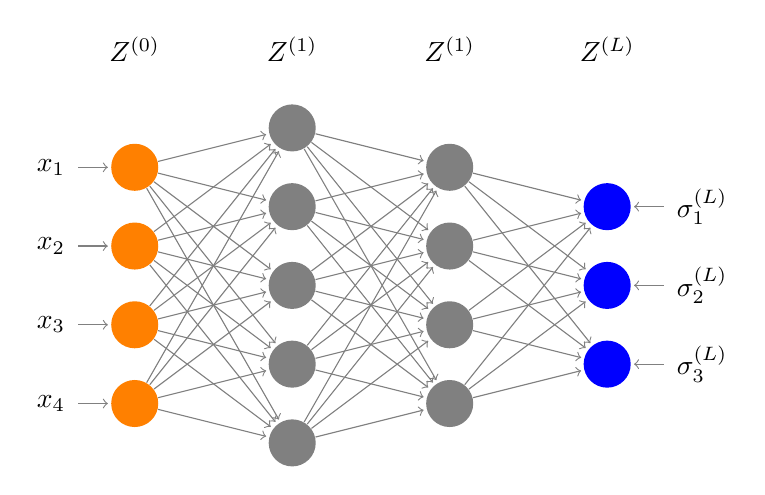
\begin{tikzpicture}[shorten >=1pt,->,draw=black!50, node distance=\layersep]
    \tikzstyle{every pin edge}=[<-,shorten <=1pt]
    \tikzstyle{neuron}=[circle,fill=black!25,minimum size=17pt,inner sep=0pt]
    \tikzstyle{input neuron}=[neuron, fill=orange];
    \tikzstyle{output neuron}=[neuron, fill=blue!100];
    \tikzstyle{hidden neuron}=[neuron, fill=black!50];
    \tikzstyle{annot} = [text width=4em, text centered]

    % Draw the input layer nodes
    \foreach \name / \y in {1,...,4}
    % This is the same as writing \foreach \name / \y in {1/1,2/2,3/3,4/4}
        \node[input neuron, pin=left: \(x_\y\)] (I-\name) at (0,-\y) {};

    % Draw the hidden layer nodes
    \foreach \name / \y in {1,...,5}
        \path[yshift=0.5cm]
            node[hidden neuron] (H1-\name) at (\layersep,-\y cm) {};
            
     \foreach \name / \y in {1,...,4}
        \path[yshift=0.5cm]
            node[hidden neuron] (H2-\name) at (2*\layersep,-0.5cm -\y cm) {};

    % Draw the hidden layer nodes
    \foreach \name / \y in {1,...,3}
        \path[yshift=0.5cm]
            node[output neuron, pin=right:\(\sigma_{\name}^{(L)}\)] (O-\name) at (3*\layersep,-1cm -\y cm) {};


    % Connect every node in the input layer with every node in the
    % hidden layer.
    \foreach \source in {1,...,4}
        \foreach \dest in {1,...,5}
            \path (I-\source) edge (H1-\dest);

    % Connect every node in the hidden layer with the output layer
    
        \foreach \source in {1,...,5}
        \foreach \dest in {1,...,4}
        \path (H1-\source) edge (H2-\dest);
    \foreach \source in {1,...,4}
        \foreach \dest in {1,...,3}
        \path (H2-\source) edge (O-\dest);

    % Annotate the layers
    \node[annot,above of=H1-1, node distance=1cm] (hl) {\(Z^{(1)}\)};
    \node[annot,left of=hl] {\(Z^{(0)}\)};
    \node[annot,right of=hl] {\(Z^{(1)}\)};
    \node[annot,above of=O-1, node distance=2cm] (ol) {\(Z^{(L)}\)};
\end{tikzpicture}
  \caption[An example of a feed-forward ANN]{An example of a feed-forward ANN,  \(\mathcal{N}\) with four layers.}
\end{figure}
The goal is to model this representation of increasing abstraction whilst maintain adjacency and full topological connectedness. Thus we construct a set of neural layers with cardinality \(L+1\), and connections as depicted in Figure 2.
    
    \begin{definition}
    
    We say $\mathcal{N}$ is a feed-forward neural network if for an input vector $\pmb{x}$,
    \[
        \begin{aligned}
        \mathcal{N}:\ & \sigma_j^{(l+1)} &= g\left(\sum_{i \in Z^{(l)}}w_{ij}^{(l)}\sigma_i^{(l)} + \beta^{(l)}\right) \\ & \sigma_j^{(1)} &= g\left(\sum_{i \in Z^{(0)}}w_{ij}^{(0)}x_i + \beta^{(0)} \right)
        \end{aligned}
    \]
    Where $1\leq l \leq L-1$. 
    \end{definition}
    
    For mathematical convenience let us denote \( \sigma_j^{(l)}\) as the output of the \(j\)\textsuperscript{th} neuron on layer \(l\). In this construction we prefer three different types of neurons, the input neuron, the hidden neuron, and the output neuron. In the case of the input neuron, there is no sigmoidal activation function, and instead we assign each \( \sigma_j^{(0)}\) to a real value which is then weighted by the dendritic input strength of each anterior neuron. Moreover an input neuron only exists on the \(0\)\textsuperscript{th} layer. In the case of each hidden layer we adopt the model described for the standard neuron as aforementioned where our sigmoid activation function \(g = \tanh(\mathrm{net})\)  is the hyperbolic tangent.%\todo{Why?}
Finally, the output layer usually have a linear sigmoid activation as to achieve output scaling beyond \([1,-1]\) in the previous layers. Once again the output layer can only exist on the layer \(L\).  
    %\todo{Personal pronouns} 

\subsection{Error Backpropagation}
   With the  functional organization of the network complete, we now need to develop the notion of learning. For the purposes of this paper we will describe a gradient descent method for learning called error-backpropagation. In the mathematical model we find conveniently that the degrees of freedom are then the dendritic weights between any two neurons. Thus these weights must be optimized against some desired output. This leads to the following multi-dimensional error function.
   \begin{definition} We call E the error function of a neural network $\mathcal{N}$, if for an input vector \(\pmb{x}\)
\[ E\left(w_{00}^{(0)}, w_{01}^{(0)}, \dots ,w_{ij}^{(L)}\right) = \frac12\sum_{i \in Z^{(L)}}{\left(\sigma_i^{(L)}-\delta_i\right)^2}\]where \(\pmb{\delta}\) is some desired output vector corresponding to \(\pmb{x}\). 
\end{definition}

Then the goal is to optimize this error function such that a reasonable local minimum is found. We then choose to modify each weight in the direction of greatest decrease for the error function. 
\begin{definition}
We call \(\pmb{\nabla}E\) the gradient of \(E\) if 
\[\pmb{\nabla}E = \left(\frac{\partial E}{\partial w_{00}^{(0)}}, 
\frac{\partial E}{\partial w_{01}^{(0)}},\dots,
\frac{\partial E}{\partial w_{ij}^{(L)}}\right)\]
for all weights, \(w_{ij}^{(l)}\), in feed-forward ANN \(\mathcal{N}\).
\end{definition}
\begin{figure}
\centering
 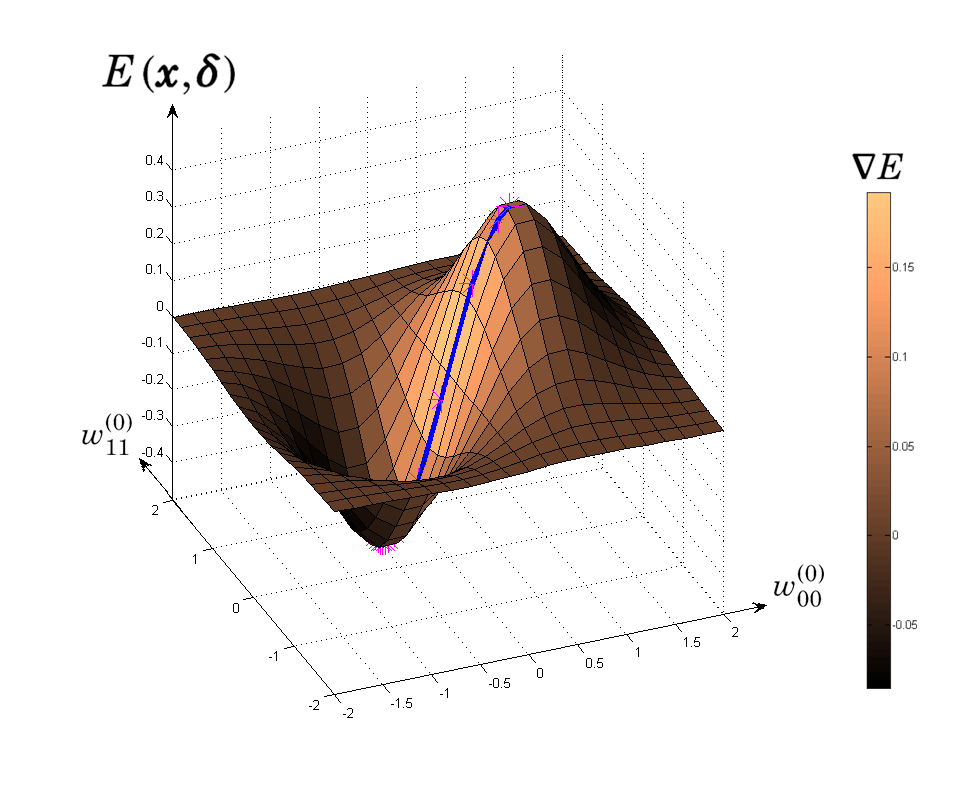
\includegraphics[width=4in]{gradient_descent}
 \caption{Gradient descent on \(E\left(\pmb{x}, \pmb{\delta}\right)\) with descent path shown in blue.}
\end{figure}
Conveniently the gradient of a function describes a vector whose direction is the greatest increase of a function. Thus to optimize our weights so that the lowest error is achieved, we update the weights as follows: \(\pmb{w}(t+1) = \pmb{w}(t)-\alpha \pmb{\nabla}E\) where alpha is some learning rate, a process which is depicted in Figure 3 \cite{rumelhart1988learning}.


The calculation of each \(\frac{\partial E}{\partial w_{ij}^{(L)}}\) is non-trivial given that each weight influences the error function in multiple ways.  To find the contribution of a single weight, recall that every single neuron is connected to all neurons in the anterior and posterior layers. So, a single weight will influence not only its posterior neuron’s sigmoidal output but also that of every neuron for any path from the posterior neuron to the set of output neurons. Thus, the multiplicity of contribution via different neural routes follows directly from the multidimensional chain-rule. Recall the differential operator \(D_g f=\frac{\partial f}{\partial x}\),
\begin{equation}
    \begin{aligned}
    \frac{\partial E}{\partial w_{ij}^{(l)}} &= D_{\sigma_0^{(L)}}\cdot D_{\mathrm{net}} \sigma_0^{(L)} \cdot D_{\sigma_0^{(L-1)}}\mathrm{net}\cdot \  \cdots \  \cdot  D_{\mathrm{net}} \sigma_j^{(l+1)} \cdot D_{w_{ij}^{(l)}}\mathrm{net} \\
    &+\  D_{\sigma_1^{(L)}}\cdot D_{\mathrm{net}} \sigma_1^{(L)} \cdot D_{\sigma_0^{(L-1)}}\mathrm{net}\cdot\  \cdots \  \cdot  D_{\mathrm{net}} \sigma_j^{(l+1)} \cdot D_{w_{ij}^{(l)}}\mathrm{net} \\
    &\ \vdots\\
    &+\  D_{\sigma_n^{(L)}}\cdot D_{\mathrm{net}} \sigma_n^{(L)} \cdot D_{\sigma_0^{(L-1)}}\mathrm{net}\cdot \  \cdots \  \cdot  D_{\mathrm{net}} \sigma_j^{(l+1)} \cdot D_{w_{ij}^{(l)}}\mathrm{net} \\
        &+\  D_{\sigma_0^{(L)}}\cdot D_{\mathrm{net}} \sigma_0^{(L)} \cdot D_{\sigma_1^{(L-1)}}\mathrm{net}\cdot \  \cdots \  \cdot  D_{\mathrm{net}} \sigma_j^{(l+1)} \cdot D_{w_{ij}^{(l)}}\mathrm{net} \\
            &\ \vdots\\
        &+\  D_{\sigma_n^{(L)}}\cdot D_{\mathrm{net}} \sigma_n^{(L)} \cdot D_{\sigma_1^{(L-1)}}\mathrm{net}\cdot \ \cdots \  \cdot  D_{\mathrm{net}} \sigma_j^{(l+1)} \cdot D_{w_{ij}^{(l)}}\mathrm{net} \\
                &\ \vdots \\
                        &+\  D_{\sigma_n^{(L)}}\cdot D_{\mathrm{net}} \sigma_n^{(L)} \cdot D_{\sigma_m^{(L-1)}}\mathrm{net}\cdot \ \cdots \ \cdot  D_{\mathrm{net}} \sigma_j^{(l+1)} \cdot D_{w_{ij}^{(l)}}\mathrm{net} \\
                        &= \sum_{a_1}^{Z^{(L)}}\ \sum_{a_2}^{Z^{(L-1)}} \cdots \sum_{a_m}^{Z^{(l+2)}} \frac{\partial E}{\partial \sigma_{a_1}^{(L)}}\frac{\partial \sigma_{a_1}^{(L)}}{\partial \mathrm{net}} \frac{\partial \mathrm{net}}{\partial \sigma_{a_2}^{(L-1)}} \ \cdots\ \frac{\partial \sigma_{a_m}^{(l+2)}}{\partial \mathrm{net}}\frac{\partial \mathrm{net}}{\partial \sigma_{j}^{(l+1)}}  \frac{\partial \sigma_{j}^{(l+1)}}{\partial \mathrm{net}} \frac{\partial \mathrm{net}}{\partial w_{ij}^{(l)}}
    \end{aligned}
\end{equation} At first sight this algorithm looks quite complicated, but a computational implementation would be able to cache certain sums and essentially reduce the complexity thereof. With the error backpropagation algorithm complete, the notion of an artificial neural network, its training, and processing is complete. Now it is possible to conjecture on variants thereof and present the primary scope of this essay.
\subsection{The Research Question}
This construction is of serious mathematical interest as feed-forward neural networks have been shown to be universal approximators; that is, they can approximate any \(f:A\to B\), where \(A,B \in \mathbb{R}^m\) are vector spaces. However it is not certain what information the approximation provides: the gradient descent algorithm does not reveal any connections between the values of the inputs.  A standing question in the field asks what can be said about the weights satisfying an approximation of $f$ besides that they exist. Therefore it is of considerable interest to explore the general form of the weights as training may not be necessary and computational complexity can be lowered.

It is the subject of this research essay to explore the neural networks through a mathematical exploration. To do this, a technique from economic mathematics is employed. It is typical that to analyze a discrete economic model, time is considered continuous and summations become integrals. To investigate neural networks then, this technique will be applied. Thus the question arises: \textbf{what can be said about artificial neural networks as the number of nodes approaches infinity and how can a real valued, continuous analogue for neural networks contribute to or aid in understanding the black box model of artificial neural networks?  }


In this paper we will generalize the notion of the universal approximation for arbitrary vector space mappings to arbitrary approximation of any \(f:L^1 (\mathbb{R}^n)\to C^\infty(\mathbb{R}^n)\) by examining the structure of feed-forward ANNs as the number of nodes for each layer becomes uncountably bounded in \(\mathbb{R}^n\). Such a generalization requires that a continuum of neural components be made, and that a continuous weight tensor or hypersurface must exist in order to maintain the topological connectedness as prescribed by the discrete model.
%!TEX root = main.tex
\section{Functional Neural Networks}

%%%%%%%%%%%%%%%%%%%%%%%%%%%%%
% INTRO                     %
%%%%%%%%%%%%%%%%%%%%%%%%%%%%%
Although neural networks have proven an extremely effective mechanism of machine learning \cite{mlsurvey}, theoretically they remain a black-box model.  In answer to this problem Neal examined the notion of infinite hidden nodes with a network proving that such a construction becomes a Gaussian kernel. Then, Roux and Bengio described a model for affine neural networks with continuous hidden layers in alignment with Neal's research. These authors showed effectively the viability of a "continuous" neural network, but left many similar constructions unexplored. It is the subject of this paper to generalize the construction of a feed-forward ANN which maps uncountably infinite vector spaces, and then to demonstrate the practical implementations of algorithms such as error backpropagation in this generalized form.

%%%%%%%%%%%%%%%%%%%%%%%%%%%%%
% DERIVATION                %
%%%%%%%%%%%%%%%%%%%%%%%%%%%%% 
\subsection{The Core Idea}
Suppose that we wish to map one functional space to another with a neural network. Consider the standard model of an ANN as the number of neural nodes for every layer becomes uncountable. The index for each node then becomes real-valued, along with the weight and input vectors 
. Let us denote \(\xi: \mathbb{R}^n\to\mathbb{R}\) as some arbitrary input function for the neural network. Likewise consider a real-valued weight function, \(w^{(l)}: \mathbb{R}^{2n}\to\mathbb{R}\), for a later $l$ which is composed of two indexing variables $i,j \in \mathbb{R}^n$. Finally as the number of neural nodes becomes uncountable we define a real-valued bound for any given layer $R^{(l)} \supset Z^{(l)}$.  As the indices become real valued, examination of the sigmoidal sum seen in definition 1.1 leads us to the following derivation.


\begin{equation}
\begin{aligned}
    \sigma^{(1)}(j) &= \lim_{\Delta i \to 0}g\left(\sum_{i\in R^{(0)}} \xi(i) w^{(0)}(i,j)\ \Delta i + \beta\right) \\
    &= g\left(\int_{R^{(0)}} \xi(i) w^{(0)}(i,j)\ di\right)
\end{aligned}
\end{equation}
The $\beta$ bias term is omitted as it can surely be formed as a constant of integration in the derivation.
Repeating the process inductively for all layers in a neural network, leads to a recurrence relation for this construction. 
\begin{definition}
We call $\mathcal{F}$ a functional neural network if,
\begin{equation}
          \begin{alignedat}{2}
        \mathcal{F}:\ &\sigma^{(l+1)}(j) & &=  g\left(\int_{R^{(l)}} \sigma^{(l)}(i) w^{(l)}(i,j)\ di \right)  \\
        &\sigma^{(0)}(j) & &= \xi(j). 
        \end{alignedat}
\end{equation}
Furthermore let $\{\mathcal{F}\}$ denote the set of all functional neural networks.
\end{definition}
To demonstrate the accuracy of this generalization, let us propose the following lemma which is near that of Roux and Bengio.
\begin{theorem} Suppose $\mathcal{F}$ is a functional neural network with a set of piecewise constant weight functions $W = \left\{w^{(0)}, w^{(1)}, \dots, w^{(L-1)}\right\}$ each with constituent pieces of length one. Then given the input function $\xi(i) = x_n, n = \max\left\{m\in \mathbb{Z}\ |\ m\leq i\right\}$ for some input vector $\pmb{x}$, $\mathcal{F}$ is discretized; that is assuming $i,j \in \mathbb{R}$ and $Z^{(l)} = R^{(l)}\ \cap \mathbb{Z}$ then for $0 \leq l \leq L-1$ we have that
\begin{equation}\mathcal{F}(\xi)= \mathcal{N}(\pmb{x})\end{equation}
\end{theorem}
\begin{proof}
Let $P(l)$ be the proposition that $\sigma^{(l+1)}(j)$ becomes discretized when $w^{(l)}(i,j)$ and $\sigma^{(l)}(i,j)$ are piecewise constant with constituent functions of length one. Moreover let $w_{ij}^{(l)}$ denote the value of $w^{(l)}(i,j)$ for $(i,j) = \max\left\{(x,y) \in \mathbb{Z}^2\ |\ x\leq i \wedge y \leq j\right\}$. Then by induction we show $P(l), 0 \leq l \leq L-1$. \\


\textit{Basis Step.} Recall that $\sigma^{(0)}(j) = \xi(j)$. Then one would suppose
\begin{equation}\sigma^{(1)}(j) = g\left(\int_{R^{(0)}} \xi(i) w^{(0)}(i,j)\ di + \beta\right)\end{equation}
but because the weight function and the input function are piecewise constant and not guaranteed to be continuous for $R^{(0)}$, we must take the improper integral along each constituent piece of length one. Supposing that each summation in the following is taken over $k\in Z^{(0)}$,
\begin{equation}
\begin{aligned}
    \sigma^{(1)}(j) &= g\left(\sum_{k}\lim_{b\to k}\int_{k-1}^b\xi(i) w^{(0)}(i,j)\ di + \beta\right) \\
    &= g\left(\sum_{k}w^{(0)}_{kj}\lim_{b\to k}\int_{k-1}^b\xi(i)\ di + \beta\right) \\
        &= g\left(\sum_{k}w_{kj}^{(0)}x_b + \beta\right)
 \end{aligned}
 \end{equation}
 
 
\textit{Inductive Step.} Now assume that for some $l$ we have that
\begin{equation}\sigma^{(l+1)}(j) = g\left(\sum_{i\in Z^{(l)}}w_{ij}^{(l)}\sigma_i^{(l)} + \beta \right)\end{equation}
We now show that by the inductive hypothesis if $P(0) \wedge P(l) \to P(l+1)$, then $P(k)\  \forall k$. Consider the next neural layer defined as
\begin{equation}\sigma^{(l+2)}(j) = g\left(\int_{R^{(l+1)}}\sigma^{(l+1)}(i) w(i,j)\ di + \beta\right)\end{equation}
Then because $w(i,j)$ and $\sigma^{(l+1)}$ are piecewise constant by definition and not necessarily continuous for $R^{(l+1)}$ we must again take the improper Riemann integral over the constituent pieces. Consider $k\in Z^{(l+1)}$
\begin{equation}
    \begin{aligned}
        \sigma^{(l+2)}(j) &= g\left(\sum_{k}\lim_{b\to k}\int_{k-1}^b\sigma^{(l+1)}(i) w(i,j)\ di + \beta\right) \\
                                          &= g\left(\sum_{k}w_{kj}^{(l+1)}\sigma_k^{(l+1)}\lim_{b\to k}\int_{k-1}^b\ di + \beta\right) \\
                                          &= g\left(\sum_{k}w_{kj}^{(l+1)}\sigma_k^{(l+1)} + \beta\right)
    \end{aligned}
\end{equation}
Therefore by the inductive hypothesis the proof follows and $\mathcal{F}(\xi) = \mathcal{N}(\pmb{x})$ for piecewise constant input and weight functions.

\end{proof}


From the logic of the preceding proof we can establish that, the input function need only be properly Lebesgue integrable over $R^{(0)}$. Moreover, we come to an extremely important intuition; the weight matrix for a given layer $l$ can be thought of as a piecewise constant weight surface, and the linear combination of weights can be thought of as a piecewise integral transformation along a given $j$ on the weight surface. However, functional neural networks allow for infinite weight surfaces and therefore can represent the entire class of integral transforms. With this in mind, it is now possible to consider functional neural networks as universal approximators.
\subsection{Universal Approximation of Bounded Linear Operators}
In the case of discretized neural networks, George Cybenko and Kolmogorov have shown that with sufficient weights and connections, a feed-forward neural network is a universal approximator of arbitrary $f:\mathbb{R}^n \to \mathbb{R}^m$ \cite{univapprox}; that is, constructs of the form $\mathcal{N}(\pmb{x})$ are dense in $C(I^n, \mathbb{R}^m)$ where $I^n$ is the unit hypercube $[0,1]^n$.  Cybenko proved this remarkable result by utilizing the Riesz Representation Theorem for Hilbert spaces and the Hahn-Banach theorem. He showed by contradiction that there exists no bounded linear functional $h(x)$ in the form of $\mathcal{N}(\pmb{x})$ such that $\int_{I_n}h(x)\ d\mu(x) = 0$.

Although this theorem has led to a remarkable interest in ANNs by legitimizing their effectiveness, it still has shed no light on the internal workings of ANNs. Fortunately using the intuitions presented in Theorem 1, it would be advantageous to examine the generalization of Cybenko's theorem to the larger class of functional neural networks. However, there is no clear way with which to do this; discretized neural networks map vector spaces and therefore approximate continuous functions, whereas functional neural networks are defined as arbitrary mappings between Hilbert spaces (more specifically the set of $L^2$ integrable functions). Moreover letting $n$ approach infinity in Cybenko's proof fails to hold in that there is not an obvious topology for $C(C(\mathbb{R}), C(\mathbb{R}))$. Therefore we must develop an approximation theorem for $\mathcal{F}: C(X) \to C(Y)$ over the set of linear operators. 

First, however, let us develop the notion of $\mathcal{F}$ as a universal approximator of arbitrary functions. By Theorem 1, we have that $\{\mathcal{F}\} \supset \{\mathcal{N}\}$ ,and in that sense for piecewise constant $w(i,j)$ and $\xi(i)$ functional neural networks approximate any arbitrary mapping from $\mathbb{R}^n \to \mathbb{R}$ where $n = |Z^{(0)}|, m = |Z^{(L-1)}|$ by Cybenko's theorem. However, when considering the fully continuous case the following corollary arises from the Stone-Weierstrass theorem.
\begin{corollary}
Suppose $\mathcal{F}$  is a multi-layer functional ANN. Then for some real-valued continuous function $f:\mathbb{R} \to \mathbb{R}$ , there exists a set of weights $W$ such that  $\forall \epsilon > 0$, $\|\mathcal{F}(\xi) - f\|_\infty < \epsilon$
\end{corollary}
\begin{proof}
In this proof we will omit the inductive step as it is elementary and employs the same logic as the basis step. Consider the first neural layer
\begin{equation}\sigma^{(1)}(j) = g\left(\int_{R^{(0)}}   \xi(i) w^{(0)}(i,j) \ di\right)\end{equation}
because we take $w^{(0)}$ to be some approximating polynomial by the Stone-Weierstrass theorem, let $w^{(0)} = \left[(g^{-1})' \circ\left(h(\Xi,j)\right)\right]h'(\Xi,j)$ approximately, where $\Xi$ is the primitive of $\xi$. Supposing that $h$ is some polynomial satisfying $h(\Xi,j)\Big|_{R^{(0)}} = f(j)$, then by the chain rule of integration
\begin{equation}
    \begin{aligned}
    \sigma^{(1)}(j) &=g\left(\int_{R^{(0)}}   \xi(i)  \left[(g^{-1})' \circ\left(h(\Xi,j)\right)\right]h'(\Xi,j)\ di\right) \\
    &= g\left(g^{-1}\left(h(\Xi,j)\right)\right)\Bigg|_{R^{(0)}} \\
    &= f(j)
    \end{aligned}
\end{equation}
\end{proof}


At this point it is important to note that the proof given above implies that $\xi$ is disregarded through manipulation of $w^{(0)}$. Instead, $h$ is a function of $\Xi$ which is the primitive of $\xi$. If we were to not let $h(\Xi,j)\Big|_{R^{(0)}} = f(j)$, then we could claim that for arbitrary $h$ we have proven any functional composition of $\xi$ is possible; that is, in some light sense we have proven Cybenko's theorem in the general case by treating the weight set as some hypersurface. Moreover, the intuition follows that if we were to discretized the satisfying $h$ and $\xi$ (Theorem 1) then it is possible that a similar weight surface is developed for a trained $\mathcal{N}$. This result is remarkable as new light is shed on the black-box model of neural networks showing that approximation of $h$ is made in the discrete sense. 


Although we have shown through the corollary that approximation of arbitrary functional composition is possible, we have yet to consider values of $w$ in the general sense. In other words, what can be said about the general approximation of bounded linear operators mapping  $C(\mathbb{R}^n)$ to $C(\mathbb{R}^n)$ where $C$ denotes the set of continuous (integrable) real valued functions? Evidently, the form of $\mathcal{F}$ resembles the general class of integral transforms, $\int f(x)\cdot E(x,k)\ dx$. Integral transforms are shown to approximate a multitude of operators through varying kernel functions. For example consider some $g(t)$ and the integral transform
\begin{equation}(\mathcal{P}g)(s) = \int_0^\infty g(t)\delta'(s-t)\ dt\end{equation}
where $\delta$ is the Dirac-Delta function. Then we have that $(\mathcal{P}g)(s) = \frac{dg}{dt}\Big|_s$ by the properties of the Delta function. Similar approximations of linear operators can be made by varying the kernel function $E$. Thus there is considerable interest in determining the density of integral transforms and thereby functional neural networks in the set of bounded linear operators.


Further investigation into dense forms of bounded linear operators leads us to the Schwartz theorem of bounded linear operator representation by integral kernels. The theorem simply states that all linear operators can be represented in some light sense by integral transforms with arbitrary kernels. However, this theorem is too general for our purposes and we would like to show that in the specific case of some functional neural network $\mathcal{F}$ that for any given layer such that $l\neq 0$ any linear operator can be approximated with point-wise convergence from the Weierstrass polynomial approximation theory.

In order to do this we will return to the Riesz representation theorem that states the following \cite{revisited}. 
\begin{theorem}
Let $\phi:C(X) \to \mathbb{R}$ be any bounded linear form where $X$ is a compact Hausdorff space and $C(X)$ is the Banach space of continuous functions over $X$. Then there exists a unique regular Borel measure $\mu$ on $X$ such that
\begin{equation}\phi(f) =\int_X f(t)\  d\mu(t),\; \; f\in C(X), \; \; t\in X\end{equation} and $\|\phi\| = |\mu|(X)$ where $|\mu|$ is the total variation of $\mu$ on $X$. 
\end{theorem}
As opposed to generalizing Cybenko's theorem to Banach spaces ($\mathbb{R}^\infty$), we can actually manipulate the representation theorem to encapsulate bounded linear operators over locally compact Hausdorf spaces. Using the aforementioned logic the universal representation theorem for functional neural networks is now proposed.
\begin{theorem}
Given a functional neural network $\mathcal{F}$ then some layer $l \in \mathcal{F}$, the let $K:C(R^{(l)})\to C(R^{(l)})$ be a bounded linear operator. If we denote the operation of layer $l$ on layer $l-1$ as $\sigma^{(l+1)} = g\left(\Sigma_{l+1}\sigma^{(l)}\right)$, then for every $\epsilon >0$, there exists a weight polynomial $w^{(l)}(i,j)$ such that the supremum norm over $R^{(l)}$ \begin{equation}\left\|K\sigma^{(l)} -\Sigma_{l+1}\sigma^{(l)}\right\|_{\infty} < \epsilon\end{equation}

\end{theorem}
\begin{proof} Let $\zeta_t :C(R^{(l)})\to R^{(l)}$ be a linear form which evaluates its arguments at $t\in R^{(l)}$; that is, $\zeta_t(f) = f(t)$.  Then because $\zeta_t$is bounded on its domain, $\zeta_t\circ K = K^\star\zeta_t$ is a bounded linear functional. Then from the Riesz Representation Theorem (Theorem 1) we have that there is a unique regular Borel measure $\mu_t$ on $R^{(l)}$ such that 
\begin{equation}
\begin{aligned}
    \left(K\sigma^{(l)}\right)(t) = K^\star \zeta_t\left(\sigma^{(l)}\right) &= \int_{R^{(l)}} \sigma^{(l)}(s)\ d\mu_t(s), \\
    \|\mu_t\| &= \|K^\star \zeta_t\| 
\end{aligned}
\end{equation}
Then if there exists a regular Borel measure $\mu$ such that $\mu_t$ is significantly smaller that $\mu$ for all $t$, then we have that, by the Radon-Nikodim derivative, $d\mu_t(s) = K_t(s)d\mu(s)$ under the assumption that $K_t$ is $L^1$ integrable over $R^{(l)}$ with the measure $\mu$. Thus it follows that 
\begin{equation}
K\left[\sigma^{(l)}\right](t) = \int_{R^{(l)}} \sigma^{(l)}(s)K_t(s)\ d\mu(s) = \int_{R^{(l)}} \sigma^{(l)}(s)K(t,s)\  d\mu(s).
\end{equation}
Therefore, for any bounded linear operator $K:C(X)\to C(X)$ there exists a unique $K(t,s)$ such that $K[f] = \int_X f(s)K(t,s) d\mu(s)$ . Now we show that the operation of $\Sigma_l$ can approximate any such operator. Because $K$ is of the form of $\Sigma_l$ where the only difference is the weighting function, we assert the following claim.

Let $G$ be defined as a linear functional applied to a Gaussian heat kernel whose application with a function $f:\mathbb{R} \to \mathbb{R}$ yields the following definition, \begin{equation}G[f](x) = \frac1{b\sqrt{\pi}}\int_\mathbb{R} f(u)\mathrm{e}^{\left(\frac{u-x}b\right)}\ du.\end{equation}Then it follows that by the Weierstrass approximation theorem that for all $\epsilon > 0$, the supremum norm $\left\|f-G[f]\right\|_\infty < \epsilon$.   Then because $G$ is a polynomial, $f$ must be a limit of polynomials. So now consider the operation of $K\left[\sigma^{(l)}\right](t)$ with kernel  $K(t,s)$. By the Weierstrass approximation theorem $K(t,s)$ must be a limit of polynomials and therefore we let $w^{(l)}(i,j)$ assume that limit. That is,
\begin{equation}
\begin{aligned}
    \lim_{b \to 0}\left\|K\left[\sigma^{(l)}\right] -  \int_{R^{(l)}} \sigma^{(l)}(s)\ G[k]\  d\mu(s) \right\|_\infty &= \\
      \left\|K\left[\sigma^{(l)}\right] -  \Sigma_{l+1}\left[\sigma^{(l)}\right]  \right\|_\infty &< \epsilon
\end{aligned}
 \end{equation}
 Thus we have that as a limit of polynomials the operation of any arbitrary layer of a functional neural network $\mathcal{F}$ approaches any arbitrary linear bounded operator $K:C(R^{(l)})\to C(R^{(l)})$; that is, functionals of the form $\Sigma_{l+1}$ are dense in the set of all bounded continuous linear operators.
\end{proof}


In the above proof, a remarkable fact has been shown: functional neural networks can perform most mathematical operations on their inputs. Consider an actual application, signal processing. If one were to employ a functional neural network for the purpose of signal classification (ie, converting audio waveforms of actual words to some digital representation like a string), the mathematical construct could perform a variety of operations such as the Fourier transform or the discrete wavelet transform, all of which are important to signal processing. More importantly, however, the approximating nature of functional neural networks is extremely valuable because it can approximate kernels ($w(i,j)$) that perform operations undiscovered by conventional mathematical methods. This advantage is similar to that of neural networks, but applicable to both discrete and continuous datasets.


Naturally, one is concerned with how those weight functions and thereby operations are developed without the preselection of priors or specific coefficients for the weight polynomials. This concern leads to the development of a training method for functional neural networks.

























\subsection{Implementation}
Now that the functional neural network has been theoretically defined, the next step is to determine whether the implementation of a numerical algorithm is possible. The problem is approached using techniques already developed for discretized networks. To produce an output for a network with $L$ layers, the implementation would propagate through all the layers while caching previous computations along the way. Likewise, for the error backpropagation method, we will cache and eliminate variables until we are able to define an algorithm that is suitably computable. 

In order to begin exploration of such an implementation, we need to both more rigorously define our notion of the weight surface and what is itself computationally evaluable.


As were for discretized neural networks, the parameters of functional neural networks are defined. In particular, the weight surface for each layer is ideally optimized for a desired output operator. To construct these weight surfaces we will parameterize them using  coefficients of Weierstrass polynomials. Consider the following definition.
\begin{definition} We say that a weight function is parameterized if it is defined as follows.
\begin{equation}
w^{(l)}(i,j) = 
    \sum_{x_{2l+1}}^{Z^{(l)}_Y} \sum_{x_{2l}}^{Z^{(l)}_X} k^{(l)}_{x_{2l},x_{2l+1}}j_{l}^{x_{2l}}j_{l+1}^{x_{2l+1}}
\end{equation}
where $k_{a,b}$ is some real valued coefficient and the order of the polynomial is arbitrary.
\end{definition}

With that in mind, let us define the notion of numerical integrability (and thereby evaluability).
% put a definition for numerical integrability
\begin{definition} \label{nint}
Let $f: \mathbb{R}^{2n}\to\mathbb{R}$, 
We say that some function $\phi$ of the form \begin{equation}\phi(x) = \int_{E\subset\mathbb{R}^n}{f(x,y)dy}\end{equation} can be numerical integrated if and only if
\begin{equation}\phi(x) = h(x)\int_{E\subset\mathbb{R}^n}/{g(y)dy}\end{equation} for some $h,g: \mathbb{R}^{n}\to\mathbb{R}$.
\end{definition}

Using the above definition we will explore the feed-forward and back-propagation actions of any given $\mathcal{F}$.












% Subsection: Fast forward Propagation
\subsubsection{Feed-Forward Propagation}

Consider the notion of numerical integrability defined in definition \ref{nint} applied to the calculation of output for some functional neural network.

\begin{theorem}
If $\mathcal{F}$ is a functional neural network with $L$ consecutive layers, then given any $l$ such that $0\leq l <  L$, $\sigma^{(l+1)}$ is numerically integrable, and if $\xi$ is any continuous and Riemann integrable input function, then $\mathcal{F}[\xi]$ is numerically integrable.
\end{theorem}

\begin{proof}
Consider the first layer. We can write the sigmoidal output of the $(l+1)^{\mathrm{th}}$ layer as a function of the previous layer; that is,
\begin{equation}
\sigma^{(l+1)} = g\left(\int_{R^{(l)}} w^{(l)}(j_l, j_{l+1})\sigma^{(l)}(j_{l})\; dj_{l}\right).
\end{equation}
Clearly this composition can be expanded using the polynomial definition of the weight surface. Hence
\begin {equation}
\begin{aligned}
\sigma^{(l+1)} &= g\left(\int_{R^{(l)}}\sigma^{(l)}(j_l)\sum_{x_{2l+1}}^{Z^{(l)}_Y}\sum_{x_{2l}}^{Z^{(l)}_X}{k_{x_{2l},x_{2l+1}}j_l^{x_{2l}}j_{l+1}^{x_{2l+1}}\;dj_l}\right) \\
&= g\left(\sum_{x_{2l+1}}^{Z^{(l)}_Y}j^{x_{2l+1}}\sum_{x_{2l}}^{Z^{(l)}_X}{k_{x_{2l},x_{2l+1}}}\int_{R^{(l)}} \sigma^{(l)}(j_l)j_l^{x_{2l}}\; dj_l\right),
\end{aligned}
\end{equation}
and therefore $\sigma^{(l+1)}$ is numerically integrable. For the purpose of constructing an algorithm, let $I^{(l)}_{x_{2l}}$ be the evaluation of the integral in the above definition for any given $x_{2l}$

It is important to note that the previous proof requires that $\sigma^{(l)}$ be Riemann integrable. Hence, with $\xi$ satisfying those conditions it follows that every $\sigma^{(l)}$ is integrable inductively. That is, because $\sigma^{(0)}$ is integrable it follows that by the numerical integrability of all $l$, $\mathcal{F}[\xi] = \sigma^{(L)}$ is numerically integrable. This completes the proof.
\end{proof}
Using the logic of the previous proof, it follows that the development of some inductive algorithm is possible. 

    
    \subsubsection{Feed-Forward Algorithm}
    Fortunately in the proof it was shown that by calculation of a constant, $I$, on each layer, the functional neural network becomes numerically integrable. The mechanism by which this can occur leads us to a simple algorithm for calculating
    $\mathcal{F}[\xi]$:
    
    \begin{enumerate}
    \item  For each $l \in \{0,\dots,L-1\}$
      \begin{enumerate}
      \item For all $t \in Z^{(l)}_X$, calculate
         \begin{equation} \label{eq:ICache} 
            I^{(l)}_t = \int_{R^{(l)}} \sigma^{(l)}(j_l)j_l^{t}\;dj_l.
         \end{equation}

       \item Calculate, for every $s \in Z^{(l)}_Y$,
         \begin{equation} \label{eq:CCache}
            C^{(l)}_{s} = \sum_{x_{2l}}^{Z^{(l)}_X} k_{x_{2l},s} I^{(l)}_{x_{2l}} 
         \end{equation}

        \item Finally, using \eqref{eq:ICache} and \eqref{eq:CCache}, cache 
          \begin{equation}
            \sigma^{(l+1)}=g\left(\sum_{x_{2l+1}}^{Z^{(l)}_Y} j^{x_{2l+1}} C^{(l)}_{x_{2l+1}}\right)
          \end{equation}
          for use in the next iteration of loop.
      \end{enumerate}
      \item The last $\sigma^{(l)}$ calculated is the output of the functional neural network.
    \end{enumerate}











% Subsection: Fast error backpropr
\subsubsection{Continuous Error Backpropagation}

Just as important as the feed-forward of neural network algorithms is the notion of training. As is common with many non-convex problems with discretized neural networks, a stochastic gradient descent method will be developed using a continuous analogue to error backpropagation. 

As is typical in optimization, a loss function is defined as follows. 
\begin{definition}
    For a functional neural network $\mathcal{F}$ and a dataset $\left\{(\gamma_n(j), \delta_n(j))\right\}$ we say that the error for a given $n$ is defined by
    \begin{equation} \label{eq:error}
        E = \frac12 \int_{R^{(L)}}\left(\mathcal{F}(\gamma_n) - \delta_n \right)^2\;dj_L
    \end{equation}
\end{definition}
This error definition follows from $\mathcal{N}$ as the typical error function for $\mathcal{N}$ is just the square norm of the difference of the desired and predicted output vectors. In this case we use the $L^2$ norm on $C(R^{(L)})$ in the same fashion.

We first propose the following lemma as to aid in our derivation of a computationally suitable error backpropagation algorithm.


\begin{lemma}
Given some layer, $l>0$, in $\mathcal{F}$, functions of the form $\Psi^{(l)} =g'\left(\Sigma_l\sigma^{(l)}\right)$ are numerically integrable. 
\end{lemma}

\begin{proof}
If\begin{equation}\Psi^{(l)}=g'\left(\int_{R^{(l-1)}}{\sigma^{(l-1)} w^{(l-1)}\ dj_{l-1}}\right)\end{equation}
then
\begin{equation}
\Psi^{(l)}=
 g'\left(
   \sum_b^{Z^{(l-1)}_Y} j_{l}^{b}
   \sum_{a}^{Z^{(l-1)}_X} k_{a,b}^{(l-1)}
    \int_{R^{(l-1)}}{\sigma^{(l-1)} j_{l-1}^a \ dj_{l-2}}
  \right)
\end{equation}
hence $\Psi$ can be numerically integrated and thereby evaluated.
\end{proof}

The ability to simplify the derivative of the output of each layer greatly reduces the computational time of the error backpropagation. It becomes a function defined on the interval of integration of the next iterated integral.

\begin{theorem}
The gradient, $\nabla E(\gamma,\delta)$, for the error function \eqref{eq:error} on some $\mathcal{F}$ can be evaluated numerically.
\end{theorem}

\begin{proof}
  Recall that $E$ over $\mathcal{F}$ is composed of $k^{(l)}_{x,y}$ for $x \in Z^{(l)}_X, y \in Z^{(l)}_Y$, and $0\leq l \leq L$.
  If we show that $\frac{\partial E}{\partial k^{(l)}_{x,y}}$ can be numerically evaluated for arbitrary, $l,x,y$, then every component of $\nabla E$ is numerically evaluable and hence $\nabla E$ can be numerically evaluated.
  Given some arbitrary $l$ in $\mathcal{F}$, let $n = L - l$.
  We will examine the particular partial derivative for the case that $n = 1$, and then for arbitrary $n$, induct over each iterated integral.

  Consider the following expansion for $n = 1$,
  \begin{align}
  \frac{\partial E}{\partial k^{(L-n)}_{x,y}} &= 
    \frac{\partial}{\partial k^{(L-1)}_{x,y}} 
    \frac{1}{2} \int_{R^{(l)}} \left[\mathcal{F}(\gamma) - \delta\right]^2\ dj_L \nonumber \\
  &= \int_{R^{(l)}} \left[\mathcal{F}(\gamma) - \delta\right] \Psi^{(L)} 
    \int_{R^{(l-1)}} j_{L-1}^x j_{L}^y \sigma^{(L-1)} dj_{L-1}\ dj_L \nonumber \\
  &= \int_{R^{(l)}} \left[\mathcal{F}(\gamma) - \delta\right] \Psi^{(L)} j_{L}^y 
    \int_{R^{(l-1)}} j_{L-1}^x \sigma^{(L-1)} dj_{L-1}\ dj_L \label{eq:n1case}
  \end{align}
  Since the second integral in \eqref{eq:n1case} is exactly $I^{(L-1)}_x$ from    \eqref{eq:ICache}, it follows that 
  
  \begin{equation}
  \frac{\partial E}{\partial k^{(n)}_{x,y}} = I^{(L-1)}_x
    \int_{R^{(l)}} \left[\mathcal{F}(\gamma) - \delta\right] \Psi^{(L)} j_{L}^y  \ dj_L
  \end{equation}
  and clearly for the case of $n=1$, the theorem holds. 

  Now we will show that this is all the case for larger $n$. 
  It will become clear why we have chosen to include $n=1$ in the proof upon expansion of the pratial derivative in these higher order cases.

  Let us expand the gradient for $n\in \{2,\dots,L\}$.
  \begin{equation} \label{eq:gradNGen}
  \begin{aligned} 
  \frac{\partial  E}{\partial k^{L-n}_{x,y}} = 
  \int_{R^{(L)}}  &[\mathcal{F}(\gamma)-\delta] \Psi^{(L)} 
   \underbrace{\int_{R^{(L-1)}} w^{(L-1)} \Psi^{(L-1)} 
  \idotsint_{R^{(L-n+1)}} w^{(L-n+1)} \Psi^{(L-n+1)}}_{n-1\text{ iterated integrals}} \\ 
    &\int_{R^{(L-n)}} \sigma^{(L-n)} j^{a}_{L-n}j^{b}_{L-n+1}\; dj_{L-n}\dots dj_L
  \end{aligned}
  \end{equation}
  As aforementioned, proving the $n=1$ case is required because for $n=1$, \eqref{eq:gradNGen} has a section of $n-1 = 0$ iterated integrals which cannot be possible for the proceeding logic.

  We now use the order invariance properly of iterated integrals (that is, $\int_A\int_B f(x,y)\;dxdy = \int_B\int_A f(x,y)\;dydx$) and reverse the order of integration of \eqref{eq:gradNGen}.

  In order to reverse the order of integration we must ensure each iterated integral has an integrand which contains variables which are guaranteed integration over some region. To examine this, we propose the following recurrence relation for the gradient. 

  Let $\{B_s\}$ be defined along $L -n \leq s \leq L$, as follows
  \begin{equation}
  \begin{aligned}
    B_L &= \int_{R^{(L)}} \left[\mathcal{F}(\gamma) - \delta\right] 
      \Psi^{(L)} B_{L-1} \;dj_L, \\
    B_s &= \int_{R^{(l)}} \Psi^{(l)}
     \sum_a^{Z^{(l)}_X} \sum_b^{Z^{(l)}_Y} j_l^a j_{l+1}^b B_{l-1} \; dj_l, \\
    B_{L-n} &= \int_{R^{(L-n)}} j_{L-n}^x j_{L-n+1}^y \; dj_{L-n}
  \end{aligned}
  \end{equation}
  such that $\frac{\partial E}{\partial k_{x,y}^{(l)}} = B_L$. If we wish to reverse the order of integration, we must find a reoccurrence relation on a sequence,
  $\{\rotB_s\}$  such that $\frac{\partial E}{\partial k_{x,y}^{(L-n)}} = \rotB_{L-n} = B_L.$ Consider the gradual reversal of \eqref{eq:gradNGen}.

  Clearly,
  \begin{equation} \label{eq:rev1}
  \begin{aligned}
    \frac{\partial E}{\partial k_{x,y}^{(l)}} =
      \int_{R^{(L-n)}}&  \sigma^{(L-n)} j^{x}_{L-n}
      \int_{R^{(L)}}[\mathcal{F}(\gamma)-\delta] \Psi^{L} 
      \int_{R^{(L-1)}} w^{(L-1)} \Psi^{(L-1)} \\ & 
      \idotsint_{R^{(L-n+1)}} j^{y}_{L-n+1}w^{(L-n+1)} \Psi^{(L-n+1)}  \; dj_{L-n+1}\dots dj_L dj_{L-n}
  \end{aligned}
  \end{equation} 
  is the first order reversal of \eqref{eq:gradNGen}. We now show the second order case with first weight function expanded.
  \begin{equation}\label{eq:rev2}
  \begin{aligned}
    \frac{\partial E}{\partial k_{x,y}^{(l)}} =
      \int_{R^{(L-n)}}&  \sigma^{(L-n)}  j^{x}_{L-n}
      \int_{R^{(L-n+1)}} \sum_b^{Z_Y} \sum_a^{Z_X} k_{a,b} j_{L-n+1}^{a+y} \Psi^{(L-n+1)}
      \int_{R^{(L)}}[\mathcal{F}(\gamma)-\delta] \Psi^{L} \\ & 
      \idotsint_{R^{(L-n+1)}} j^b_{L-n+2} w^{(L-n+2)} \Psi^{(L-n+2)}  \; dj_{L-n+1}\dots dj_L dj_{L-n}.
  \end{aligned}
  \end{equation}

  Repeated iteration of the method seen in \eqref{eq:rev1} and \eqref{eq:rev2}, where the inner most integral is moved to the outside of the $(L-s)^\mathrm{th}$ iterated integral, with $s$ is the iteration, yields the following full reversal of \eqref{eq:gradNGen}. For notational simplicity recall that $l = L-n$, then
 \begin{equation}\label{eq:revn}
  \begin{aligned}
    \frac{\partial E}{\partial k_{x,y}^{(l)}} =&
      \int_{R^{(l)}}  \sigma^{(l)}  j^{x}_{l}
      \int_{R^{(l+1)}} \sum_a^{Z^{(l+1)}_X} j_{l+1}^{a+y} \Psi^{(l+1)}
      \int_{R^{(l+2)}} \sum_b^{Z_Y^{(l+1)}} \sum_c^{Z_X^{(l+2)}}
         k^{(l+1)}_{a,b} j^{b+c}_{l+2} \Psi^{(l+2)} \\&
      \int_{R^{(l+3)}} \sum_d^{Z_Y^{(l+2)}} \sum_e^{Z_X^{(l+3)}}
         k^{(l+2)}_{c,d} j^{d+e}_{l+3} \Psi^{(l+3)} 
      \idotsint_{R^{(L)}} \sum_q^{Z^{(L-1)}_Y} k^{(L-1)}_{p,q} j_L^q 
       \; [\mathcal{F}(\gamma)-\delta] \Psi^{(L)} \\ &
      \qquad \qquad dj_{L}\dots dj_{L-n}.
  \end{aligned}
  \end{equation}

  Observing the reversal in \eqref{eq:revn}, we yield the following recurrence relation for $\{\rotB_s\}$. Bare in mind, $l= L-n$, $x$ and $y$ still correspond with $\frac{\partial E}{\partial k^{(l)}_{x,y}}$, and the following relation uses its definition on $s$ for cases not otherwise defined.
  \begin{equation} \label{eq:rotBrelation}
  \begin{aligned}
    \rotB_{L,t} &= \int_{R^{(L)}}  \sum_b^{Z^{(L-1)}_Y} k^{(L-1)}_{t,b} j_L^b 
      \left[\mathcal{F}(\gamma) - \delta\right] \Psi^{(L)}\;dj_L. \\
    \rotB_{s,t} &= \int_{R^{(s)}}\sum_b^{Z^{(s-1)}_Y} \sum_a^{Z^{(s)}_X} 
      k^{(s-1)}_{t,b} j_s^{a+b} \Psi^{(s)} \rotB_{s+1,a}\; dj_s. \\
    \rotB_{l+1} &= \int_{R^{(l+1)}} \sum_a^{Z^{(l+1)}_X}
      j^{a+y}_{l+1} \Psi^{(l+1)} \rotB_{l+2, a}\; dj_{l+1}. \\
     \frac{\partial E}{\partial k^{(l)}_{x,y}} = \rotB_{l} &= \int_{R^{(l)}}
      j_{l}^x \sigma^{(l)} \rotB_{l+1}\; dj_l.
  \end{aligned}
  \end{equation}
  Note that $\rotB_{L-n} = B_L$ by this logic.

  With \eqref{eq:rotBrelation}, we need only show that $\rotB_{L-n}$ is integrable. Hence we induct on $L-n \leq s \leq L$ over $\{\rotB_s\}$ under the proposition that $\rotB_s$ is not only numerically integrable but also constant. 

  Consider the base case $s = L$. For every $t$,
  because every function in the integrand of $\rotB_L$ in \eqref{eq:rotBrelation} is composed of $j_L$, functions of the form $\rotB_L$ must be numerically integrable and clearly, $\rotB_L \in \mathbb{R}$.

  Now suppose that $\rotB_{s+1,t}$ is numerically integrable and constant. Then, trivially, $\rotB_{s,u}$ is also numerically integrable by the contents of the integrand in \eqref{eq:rotBrelation} and $\rotB_{s,u} \in \mathbb{R}$. Hence, the proposition that $s+1$ implies $s$ holds for $l+1 < s < L$.

  Lastly we must show that both $\rotB_{l+1}$ and $\rotB_{l}$ are numerically integrable. By induction $\rotB_{l+2}$ must be numerically integrable. Hence by the contents of its integrand $\rotB_{l+1}$ must also be numerically integrable and real. As a result, $\rotB_l =  \frac{\partial E}{\partial k^{(l)}_{x,y}}$ is real and numerically integrable.

  Since we have shown that $ \frac{\partial E}{\partial k^{(l)}_{x,y}}$ is numerically integrable, $\nabla E$ must therefore be numerically evaluable as aforementioned. This completes the proof.
\end{proof}


\subsubsection{Continuous Error Backpropagation Algorithm}
The logic of the proceeding proof required the establishment of $\{\rotB_s\}$ as a sequence with a recurrence relation defining each component of the gradient on some coefficient in the network. Interestingly enough for $L$ large enough certain elements of $\{\rotB_s\}$ can be reused for different $n$. In order to more accurately describe this process, we propose the following algorithm for calculating gradients in stochastic gradient descent. \\

\begin{enumerate}
\item For all $\lambda \in \{ 1,\dots, L \}$, calculate $\Psi^{(\lambda)}$.

\item Calculate $K - \nabla E \to K$ where $K$ is the vector of all coefficient matrices by calculating each partial matrix over $l \in \{0,\dots, L-1\}$

  \begin{enumerate}
  \item If $l = L - 1 \Leftrightarrow (n = 1)$, then store into the coefficient matrix
    \begin{equation}
       k_{x,y}^{(L-1)} - I_x^{(L-1)}
        \int_{R^{(L)}} \left[\mathcal{F}(\gamma) - \delta\right] 
          \Psi^{(L)} j_L^y \; dj_L \to  k_{x,y}^{(L-1)}
    \end{equation}
    for every $x,y.$
    

    \item  If $l < L - 1 \Leftrightarrow n > 1$, then
    \begin{enumerate}
      \item Ensure that $\rotB_{l+2,t}$ from \eqref{eq:rotBrelation} is computed for all $t \in Z^{(l+1)}_X$

      \item Then for all $x\in Z^{(l)}_X$ and $y\in Z^{(l)}_Y$,
      \begin{enumerate}

        \item Compute
          \begin{equation}
           \rotB_{l+1} = \int_{R^{(l+1)}} \sum_a^{Z^{(l+1)}_X}
             j^{a+y}_{l+1} \Psi^{(l+1)} \rotB_{l+2, a}\; dj_{l+1}. 
          \end{equation}

        \item Compute 
        \begin{equation}
           \frac{\partial E}{\partial k^{(l)}_{x,y}} = \rotB_{l} = \int_{R^{(l)}}
            j_{l}^x \sigma^{(l)} \rotB_{l+1}\; dj_l.
        \end{equation}
      
        \item Update the weights such that 
        \begin{equation}
          k_{x,y}^{(l)} - \rotB_l \to k_{x,y}^{(l)}
        \end{equation}
      \end{enumerate}
    \end{enumerate}
  \end{enumerate}
\end{enumerate}

With the completion of the implementation, the theoretical definition of functional neural networks is complete.
%!TEX root = main.tex

\section{Generalized Artificial Neural Networks}



We have clearly demonstrated the theoretical power of FNNs, but does there exist some more general structure which includes FNNs and ANNs without piecewise approximation? In other words, can we determine a form which encompasses the discrete classification of continuous datasets or visa versa all the while maintains either the power of discrete or functional artificial neural networks? The solution to such questions must furthermore maintain universal approximation and computational evaluability so as to allow the implementation of a real-world algorithm. 

In this section of the paper we will propose the Generalized Artificial Neural Network through the examination of specific operations on different layers. 

\subsection{The Generalization of ANNs}
In order to generalize ANNs in a way that follows logically, we take the initial definition of functional neural networks and consider the notion of a layer.
\begin{definition} If $A,B$ are (possibly distinct) Hilbert spaces over $\mathbb{R}$,
we say $\mathcal{G}: A \to B$ is a generalized neural network if and only if 

\begin{equation} \label{eq:gann}
          \begin{alignedat}{2}
        \mathcal{G}:\ &\sigma^{(l+1)} & &=  g\left(T_l\left[\sigma^{(l)}\right] + \beta^{(l)}\right)  \\
        &\sigma^{(0)} & &= \xi 
        \end{alignedat}
\end{equation}
for some input $\xi \in A$.
\end{definition}

In \eqref{eq:gann}, it is unclear how the form of $T_l$ is restricted. It might be recalled that $T_l$ takes a form similar to the operation of a layer $l+1$ on $l$ in the proof of universal approximation for $\{\mathcal{F}\}$. Let us consider a few other such forms of $T_l$ by first stating a formal definition.

\begin{definition}
We say that $T_l$ is the operation of a layer $l+1$ on $l$ in some $\mathcal{G}$ if and only if for $l=L-1$, $T:C\to B$ with $C$ the codomain of $\sigma^{(0)}$ and for $l = 0$, $T_l : A\to D$ where $D$ is the domain of $\sigma^{(1)}.$
\end{definition}

Using the above definition it is now possible to construct different classes of $T_l$ using ideas directly from the constructions of $\mathcal{N}$ and $\mathcal{F}$.

\begin{definition}
We suggest several classes of $T_l$ as follows
	\begin{itemize}
	\item $T_l$ is said to be $\mathfrak{f}$ functional if and only if 
		\begin{equation} \label{eq:tlfunctional}
		\begin{aligned} 
			T_l = \mathfrak{f}: C(R^{(l)}) \to&\ C(R^{(l+1)}) \\
			\sigma(i) \mapsto& \int_{R^{(l)}} \sigma(i) w^{(l)}(i,j)\ di.
		\end{aligned}
		\end{equation}
	\item $T_l$ is said to be $\mathfrak{n}$ discrete if and only if 
		\begin{equation} \label{eq:tldiscrete}
		\begin{aligned} 
			T_l = \mathfrak{n}: \mathbb{R}^n \to&\ \mathbb{R}^m \\
			\vec{\sigma} \mapsto& \sum_j^m \vec{e}_j\sum_i^n \sigma_i w^{(l)}_{ij}
		\end{aligned}
		\end{equation}
		where $\vec{e}_j$ denotes the $j^\mathrm{th}$ basis vector in $\mathbb{R}^m$.
	\item $T_l$ is said to be $\mathfrak{n}_1$ transitional if and only if 
		\begin{equation} \label{eq:tldiscrete}
		\begin{aligned} 
			T_l = \mathfrak{n}_1: \mathbb{R}^n \to&\  C(R^{(l+1)}) \\
			\vec{\sigma} \mapsto& \sum_i^n \sigma_i w^{(l)}_i(j).
		\end{aligned}
		\end{equation}
	\item $T_l$ is said to be $\mathfrak{n}_2$ transitional if and only if 
		\begin{equation} \label{eq:tldiscrete}
		\begin{aligned} 
			T_l = \mathfrak{n}_2: C(R^{(l)}) \to&\ \mathbb{R}^m \\
			\sigma(i) \mapsto& \sum_j^m \int_{R^{(l)}} \sigma(i) w^{(l)}_j(i)\ di
		\end{aligned}
		\end{equation}
	\end{itemize}
\end{definition}

With the characterization of these layer classes complete, foundational theorems about this new generalization must be proposed. First we will show inclusion of other neural algorithms followed by universal approximation theorems (as by necessesity). 

\begin{theorem}
If $\{\mathcal{G}\}$ is the set of all generalized artificial neural networks then $\{\mathcal{F}\} \cup \{\mathcal{N}\}$ is a subset of $\{G\}$.
\end{theorem}
\begin{proof}
Since $\{\mathcal{N}\} \subset \{\mathcal{F}\}$, we need only show that $\{\mathcal{F}\} \subset \{\mathcal{G}\}$, but for the sake of the reader, consider that one might take any $\mathcal{N}$ and show equivalency with some $\mathcal{G}$ strictly composed of $T_l$ which are discrete.

For the case of functional inclusion, consider any functional neural network $\mathcal{F}$ with $L$ layers. Then let us construct $\mathcal{G} : C\left(R^{(0)}\right) \to C\left(R^{(L)}\right)$. First we endow $\mathcal{G}$ with $T_l$ which are strictly functional. Let each $T_l$ have an equivalent weight function $w^{(l)}$ to that of $\mathcal{F}$ on layer $l$. This construction yields the following reccurrance relation:
\begin{equation}
          \begin{alignedat}{2}
        \mathcal{G}:\ &\sigma^{(l+1)}(j) & &=  g\left(\int_{R^{(l)}} \sigma^{(l)}(i) w^{(l)}(i,j)\ di + \beta^{(l)}\right)  \\
        &\sigma^{(0)}(j) & &= \xi(j), 
        \end{alignedat}
\end{equation}
which is exactly equivalent to that of $\mathcal{F}$. Hence for any $\mathcal{F}$ there exists a corresponding $\mathcal{G}$ with equivalency. Thus $\{\mathcal{F}\} \subset \{\mathcal{G}\}.$
\end{proof}
%!TEX root = main.tex
\section{Conclusion}
When the research question was posed, the goal was to develop a mathematical construct that is continuously homologous to standard and discrete artificial neural networks. This along with inspiration from common economic techniques like interpolation led us to consider a neural network structure containing infinite input, hidden, and output neurons. This new construction is named the functional neural network and has the same properties as discrete neural networks.

The proposition of functional neural networks lead to new insights into the black box model of traditional neural networks. First, functional networks are a logical generalization of the discrete neural network and therefore all theorems shown for traditional neural networks apply to piecewise functional neural networks. Furthermore the creation of homologous theorems for universal approximation provided a way to find a relationship between the weights of traditional neural networks. This suggests that the discrete weights of a normal artificial neural network can be transformed into continuous surfaces which approximate kernels satisfying the training dataset. Functional neural networks are also able to approximate bounded linear operators (the general form of functions), homologous to how ANNs apprxoimate functions. Finally a continuous version of the error backpropagation algorithm was developed, providing information into how the discrete error backprop algorithm operates: the chain rule just becomes convolution integration across partially derived anterior layers.

These algorithms, while theoretically feasible, were originally too computationally complex to have a practical application. The algorithms were reapproached mathematically to make feed forward and error backpropagation numerically integrable.  This property is shown through the expansion of the weight polynomial and the interchanging of iterated integrals. From this, a computational implementation of the new generalized construct, FNNs, is created. Furthermore, the process of caching important values in weight coefficient calculation greatly reduced the original factorial complexity such that the algorithms could run in reasonable computational time.

Thus, the functional neural network not only provides novel mathematical insights behind the traditional neural network algorithm, it also becomes a feasible new machine learning method. This new field has many potential directions especially with continued techniques from mathematical analysis.

\subsection{Future Work}
The computational algorithm was applied to analyze the Laplace transform. However, there is still a range of applications to be explored. The original intent of this paper was to explore continuous data that exists in the real world. Sound waves and sight analysis by ears and eyes occurs on a continuous level yet most of the data analysis in these fields has discretized the data for numerical evaluation. The insertion of continuous sinusoidal definition of these datasets into a FNN would be a possible field of exploration.

On the theoretical side, it must be proven, or disproven, that functional neural networks are or are not analytically integrable in closed form. If they are integrable then the aforementioned computational implementation will be very simple and possibly faster than discrete neural networks. In the case that they are not, functional neural networks may remain simply a theoretical construct for understanding discrete neural networks. Evidence has been shown that it is integrable using a linear sigmoid activation functions. However, for nonlinear sigmoid activation functions, there is a strong indication that there is no closed form interval solution.

\newpage
\addcontentsline{toc}{section}{Works Cited}
\printbibliography

\end{document}